\documentclass[default]{subfiles}

\addbibresource{cite.bib}

\begin{document}
\selectlanguage{english}

\graphicspath{{image/}}

\udc{} % TODO
\pacs{} % TODO
\edn{} % TODO

\documentType{Review}

\title{Reconstructing the Volumetric Geometry of the Cerebral Cortex Based on Magnetic Resonance Imaging}

\author[rudn, prmu]{Ivan V. Brak}
\author[rudn]{Konstantin G. Leladze}
\author[rudn]{Gleb A. Kiselev}

\address[rudn]{RUDN University, 6 Miklukho-Maklaya St, Moscow, 117198, Russian Federation}

\address[prmu]{Privolzhsky Research Medical University, 178T Gagarina Ave., Nizhny Novgorod, Russia, 603107}
  
\received{31}{12}{2025} % TODO
\revised{31}{12}{2025} % TODO
\accepted{31}{12}{2025} % TODO

\begin{authordescription}
  \authorfull[english]{Brak, Ivan V.}
  \authordegree[english]{Candidate of Biology Sciences}
  \authorpost[english]{
    Senior Lecturer at the Department of Mathematical Modeling and Artificial Intelligence of
    Peoples' Friendship University of Russia (RUDN University); Researcher of Privolzhsky Research Medical University
  }
  \email{i.v.brak@gmail.com}
  \orcid{0000-0002-5146-0096}
  \researcherid{AAM-4659-2021}
  \scopusauthorid{24461311200}
  \phone{+7(913)2072333}
\end{authordescription}

\begin{authordescription}
    \authorfull[english]{Leladze, Konstantin G.}
    \authorpost[english]{
      PhD student of Department of Mathematical Modeling and Artificial Intelligence of  Peoples' Friendship University
      of Russia (RUDN University)
    }
    \email{1142230347@pfur.ru}
\end{authordescription}

\begin{authordescription}
  \authorfull[english]{Kiselev, Gleb A.}
  \authordegree[english]{Candidate of Technical Sciences}
  \authorpost[english]{
    Senior Lecturer at the Department of Mathematical Modeling and Artificial Intelligence of
    Peoples' Friendship University of Russia (RUDN University); Researcher of Federal Research Center "Computer
    Science and Control" of the Russian Academy of Sciences
  }
  \email{kiselev@isa.ru}
  \orcid{00000-0001-9231-8662}
  \researcherid{Y-6971-2018}
  \scopusauthorid{57195683637}
  \phone{+7(906)7993329}
\end{authordescription}

\abstracts{
    This review article focuses on the analysis of approaches for reconstructing the volumetric geometry of the
    cerebral cortex and white matter tracts based on magnetic resonance imaging (MRI) data. Particular attention is
    given to voxel-based morphometry (VBM) and surface-based morphometry (SBM) — two key methodologies for the
    quantitative analysis of brain structure. The algorithmic principles of each method are considered, along with
    their advantages, limitations, and metric characteristics, including cortical thickness, surface area, and
    gyrification index.

    A separate focus is placed on comparing the sensitivity and accuracy of VBM and SBM in identifying morphological
    changes related to cognitive and neuropsychiatric traits. Additionally, the article discusses the promising
    tensor-based surface morphometry (TBSM), which is based on differential geometry methods and provides high spatial
    resolution without topological distortion.

    This work emphasizes the importance of accurate and reproducible structural brain reconstruction in the context of
    biomedical technology and neuroscience development.
}

\keywords{
  brain morphometry, SBM, VBM, cortical thickness, MRI, anatomical reconstruction, neuroimaging reproducibility
}

\alttitle{Восстановление объемной геометрии коры головного мозга по результатам магнитно резонансной томографии}

\altauthor[rudn, prmu]{И. В. Брак}
\altauthor[rudn]{Г. А. Киселёв}
\altauthor[rudn]{К. Г. Леладзе}

\altaddress[rudn]{Российский университет дружбы народов, ул. Миклухо-Маклая, д.6, Москва, Россия, 117198}
\altaddress[prmu]{
  Приволжский исследовательский медицинский университет, пр. Гагарина, д. 178Т, Нижний Новгород, Россия, 603107
}

\altabstracts{
    Настоящая обзорная статья посвящена анализу подходов к восстановлению объемной геометрии коры головного мозга и
    проводящих путей на основе данных магнитно-резонансной томографии. Основное внимание уделено
    воксельно-ориентированной (VBM) и поверхностно-ориентированной (SBM) морфометрии — двум ключевым направлениям в
    количественном анализе структуры мозга. Рассматриваются алгоритмические принципы каждого подхода, их достоинства,
    ограничения, а также метрические характеристики, включая толщину коры, площадь поверхности и индекс гирификации.
    
    Отдельный акцент сделан на сравнении чувствительности и точности VBM и SBM в выявлении морфологических изменений,
    связанных с когнитивными и нейропсихическими особенностями. Также рассматривается перспективный
    тензорно-ориентированный подход (TBSM), опирающийся на методы дифференциальной геометрии и обеспечивающий высокую
    разрешающую способность без искажения топологии.
    
    Работа подчёркивает значимость точной и воспроизводимой структурной реконструкции мозга в контексте развития
    биомедицинских технологий и нейронауки.
}

\altkeywords{
  морфометрия мозга, SBM, VBM, толщина коры, МРТ, анатомическая реконструкция, воспроизводимость нейровизуализации
}

\maketitle

\section{Purpose of the Article}

The purpose of this article is to review existing approaches to modeling brain tissue using MRI data and to identify
the key criteria for evaluating the reliability of these models. Special attention is paid to international
collaborations, their standards, algorithms, and impact on the reproducibility of neuroimaging research.

\section{Introduction}

\label{sec:intro}

Understanding the structure of the human brain is key to deciphering the physical basis of cognitive functions, mental
disorders, and individual differences. Reconstructing an accurate volumetric geometry of the cortex and white matter
tracts is not only a technical challenge but also a foundation for a new neuroscience — quantitative, reproducible, and
scalable. Modern methods make it possible to reconstruct the three-dimensional morphology and topology of gray and
white matter with high resolution based on MRI data, which is fundamentally important for clinical diagnostics,
neuroscience, and cognitive research.

To ensure the accuracy and reproducibility of studies, international consortia and national initiatives have been
established, which define the standards for processing and analyzing neuroimaging data. 

\section{International Collaborations in Neuroimaging}

In recent years, an increasing number of international organizations and consortia have emerged, focusing on brain
research based on morphometric data. Some of the most notable include:

\begin{itemize}
    \item ENIGMA Consortium — one of the world’s largest international neuroimaging consortia, comprising over 1,400
    scientists from 50 countries. ENIGMA aggregates data from thousands of studies to conduct meta-analyses,
    particularly in the fields of psychiatric disorders, brain genetics, and neurodevelopment. The consortium develops
    standardized protocols for segmentation, normalization, and cortical reconstruction based on MRI data, making its
    approaches a benchmark in the field \cite{hellard_2014}.

    \item Human Connectome Project (HCP) — an interdisciplinary initiative funded by the NIH, aimed at creating the
    most accurate map of human brain connectivity. The project uses multimodal MRI data (structural, functional, and
    diffusion MRI) and develops algorithms for white matter tract and cortical geometry reconstruction with a
    resolution of up to 0.7 mm3 \cite{van_2013}.
    
    \item Brainnetome Project — a Chinese initiative that has developed a functional-anatomical parcellation of the
    brain based on MRI and connectivity data \cite{milton_2021}. Brainnetome provides a detailed database with
    high-precision reconstructions of cortical and subcortical structures and their connections
    \cite{jiang_2013, hohnson_2016}.
    
    \item CHIMGEN (China Imaging Genetics Project) — a Chinese project that employs structural and functional
    neuroimaging, genetic analysis, and psychometric testing to build brain models that account for both genetic and
    environmental factors \cite{xu_2020}.
    
    \item SRPBS (Strategic Research Program for Brain Sciences) — a Japanese national initiative supporting the
    development of neuroimaging technologies, including high-resolution 3D brain reconstruction, automated segmentation
    tools, and the application of AI for neural structure analysis (Kawato, 2015).
    
    \item COCORO (Cognitive Genetics Collaborative Research Organization) — a Japanese multicenter project focusing on
    cognitive disorders and the reconstruction of cortical morphology in patients with psychoses, schizophrenia
    \cite{madeira_2020}, and bipolar disorder \cite{koshiyama_2022}.\newline
\end{itemize}

These projects not only define standards for data acquisition and processing but also provide accessible databases,
analysis tools, and software environments (e.g., FreeSurfer \cite{caser_2024}, FSL, BrainSuite), enabling researchers
worldwide to reproduce reconstructions and conduct comparative studies.

However, despite these achievements, a critical evaluation of the employed methodologies remains essential — from
voxel- and surface-based morphometry to more complex probabilistic models based on machine learning and deep learning.
Even minor artifacts or preprocessing biases can affect the topology of the reconstructed model, and the use of AI may
amplify systematic errors. Therefore, the accuracy of structural reconstruction becomes a critical factor in
establishing trust in the conclusions of neuroimaging analysis.

\section{Morphometric Analysis of the Human Brain}

Brain morphometry refers to a set of quantitative methods aimed at measuring the geometric characteristics of brain
structures based on neuroimaging, most commonly magnetic resonance imaging (MRI). Unlike visual assessment, the
morphometric approach enables numerical evaluation of volume \cite{upadhyay_2014, fischl_2012, wang_2019, makris_2006},
Thickness \cite{upadhyay_2014, fischl_2000, fischl_2012, wang_2019, makris_2006}, surface area
\cite{desikan_2006, fischl_2012, fischl_2004, wang_2019, makris_2006}, and curvature
\cite{fischl_2012, fischl_2000, wang_2019, makris_2006} of various brain regions, as well as their spatial arrangement
(topography) \cite{desikan_2006, fischl_2008, fischl_1999, wang_2019} and symmetry
\cite{desikan_2006, greve_2013, fischl_2004, wang_2019}. These metrics \cite{klein_2017} become particularly
important for identifying both individual and group-level differences — within the normative range and in
neurodegenerative and neuropsychiatric conditions, such as Alzheimer's dicease \cite{he_2024}, depressive
\cite{van_2013} and schizotypal disorders.

One of the key objectives of morphometry is the construction of anatomically accurate, reproducible, and comparable
brain models suitable for both fundamental research and clinical diagnostics. Differences in the morphology of the
cortex, subcortical structures, and white matter tracts can reflect a wide spectrum of cognitive, behavioral, and
pathological characteristics. For example, the works by Sao et al. \cite{cao_2023} and Fischl et al. \cite{fischl_2000}
clearly demonstrate how variations in cortical thickness — both global and local patterns — can predict cognitive
status and disease; and study \cite{shaw_2006} shows that the trajectory of cortical thickness changes correlates with
cognitive abilities (memory, attention, executive functions). In \cite{jagger_2018}, it is shown that reductions in
gray matter volume in the caudate nucleus and prefrontal cortex in children and adolescents negatively affect executive
functioning and cognitive control, which complicates academic performance.

Beyond its diagnostic utility, morphometry plays an important role in understanding the principles of brain
organization. When combined with behavioral, genetic, and psychometric data, it enables the identification of links
between brain anatomy and function, between biology and psyche. This is especially relevant in the era of big data,
where current scientific organizations and consortia are working to identify reproducible patterns of brain
organization across thousands and tens of thousands of subjects, developing new — including stochastic — methods for
their detection \cite{daoudi_2024, kurella_2023, cruz_2021, mosch_2023}.

Moreover, morphometric techniques form the foundation of modern approaches to building digital twins of the brain —
high-precision models that are becoming increasingly relevant with the integration of artificial intelligence
technologies into medicine. The reliability of such models depends on the accuracy of morphometric analysis, the
quality of input data, and the correctness of the algorithms used. Therefore, the development and evaluation of
morphometric methods is a critical task not only for neuroscience but also for the entire biomedical technology
industry \cite{marteua_2024, xiong_2023}.

This article reviews the principal approaches to cortical brain morphometry: voxel-based and surface-based, as well as
the data quality criteria and processing pipelines that determine the reliability of cortical reconstruction results.

\section{MRI-Based Morphometric Approaches to Brain Reconstruction}

The standard approaches in morphometric analysis are voxel-based and surface-based morphometry. Both allow for the
assessment of structural brain changes. Voxel-based morphometry analyzes tissue volume at the voxel level, while
surface-based morphometry focuses on cortical surface characteristics such as thickness and curvature. Both methods
operate within a single spatial scale and do not detect patterns emerging at different levels of organization, which
limits their analytical power \cite{cao_2023}.

\subsection{Voxel-Based Morphometry}
Voxel-Based Morphometry (VBM) is a technique for quantitatively assessing anatomical differences in the brain by
analyzing brain tissue structure directly in the volume of three-dimensional MRI data at the voxel level.

The general VBM processing pipeline includes the following steps:\newline

\begin{enumerate}
    \item The VBM workflow begins with spatial normalization, in which individual MRI scans are transformed into a
    standard anatomical space \cite{desikan_2006}. This is achieved using non-linear registration algorithms based on
    image intensities and anatomical templates, allowing for the alignment of corresponding brain regions across
    individuals.
    
    \item At the next stage, tissue segmentation is performed, dividing brain tissue into major classes: gray matter,
    white matter, and cerebrospinal fluid. This step employs classification algorithms, most commonly based on
    statistical modeling of voxel intensity values and their spatial characteristics.
    
    \item  The segmented images then undergo spatial smoothing, which increases the sensitivity of statistical analysis
    by reducing inter-subject variability in the localization of specific structures.
    
    \item  In the final step, statistical analysis is carried out to compare the volumes or densities of gray matter at
    the voxel level either between subject groups or in relation to a continuous variable. The output is a statistical
    map highlighting brain regions with significant structural differences.\newline
\end{enumerate}


Thus, the VBM pipeline enables automated and objective comparison of anatomical features directly from 3D MRI data,
bypassing the surface reconstruction stage that is characteristic of surface-based morphometry.

\subsection{Surface-Based Morphometry}
Surface-Based Morphometry (SBM) is an MRI analysis approach focused on the geometry and metrics of the cortical
surface. There are several key variations and techniques implementing SBM, differing in analytical goals, types of
metrics, and underlying algorithms \cite{riccelli_2017}.

SBM is frequently employed for morphometric reconstruction. For instance, study \cite{desikan_2006} describes the use
of this approach for automated segmentation of the cerebral cortex based on structural magnetic resonance imaging data.
The input consists of high-quality T1-weighted brain MRI scans, which are first subjected to artifact correction,
intensity normalization, skull stripping, and generation of a three-dimensional model of the gray–white matter
boundary.

In SBM, cortical surface reconstruction is performed such that each MRI volume is represented as an inflated
("unfolded") surface of the brain, allowing access to structures typically hidden within sulci and gyri. A critical
requirement for the input images is high spatial resolution (approximately 1 mm voxel size), minimal motion artifacts,
and clear contrast between gray and white matter. Cortical surfaces are matched to one another via mapping to a
spherical template \cite{fujita_2019}, followed by automatic registration based on curvature and the geometry of sulcal
and gyral patterns \cite{li_2023}.

The outputs of the SBM approach are anatomically accurate maps delineating cortical regions of interest, each
corresponding to specific gyri or sulci. In \cite{desikan_2006}, 34 such regions were automatically labeled in each
hemisphere. These maps exhibit high precision and reproducibility: the average spatial discrepancy between automated
and manual labeling does not exceed one millimeter, and the intraclass correlation coefficient (ICC) is approximately
0.835, indicating strong agreement and validity of the developed method. These results highlight the effectiveness of
SBM in both research and clinical contexts that require precise and reproducible anatomical localization on the
cortical surface.

Like VBM, SBM is highly dependent on the quality of the input data. Study \cite{fischl_2012} explores surface-based
morphometry in depth, with an emphasis on cortical surface reconstruction and cortical thickness estimation. A central
focus is the correction of topological defects that arise during cortical surface reconstruction from MRI data. As in
\cite{desikan_2006}, the input consists of T1-weighted brain MR images, which must meet high spatial resolution
requirements and demonstrate stable intensity characteristics. However, the method is also capable of adapting to
intensity variations caused by histological differences and scanner artifacts.

A notable innovation described in the study is the approach to correcting surface topology. Rather than attempting to
construct a surface with an assumed correct topology from the outset, the authors begin with a surface that may contain
defects and iteratively transform it into a spherical shape. This process enables identification of regions with
topological errors, which are then locally corrected. This technique significantly improves the geometric accuracy of
the reconstructed model and reduces manual labor, thereby enhancing the automation of the surface reconstruction
process and making it suitable for large-scale clinical and research studies \cite{yotter_2011}.

The output of this method is an accurate model of the cortical surfaces, including both the inner (gray–white matter
boundary) and outer (pial) surfaces. A key outcome is the high accuracy of cortical thickness measurements — reaching a
resolution of less than a quarter millimeter — confirmed by multiple validation studies, including comparison with
histological data. This enables the detection of morphometric changes associated with various pathological conditions,
age-related differences, or neuropsychological traits with exceptionally high sensitivity and reproducibility
\cite{has_2016}.

SBM Results Enable, in Particular, the following:
\begin{itemize}
    \item Analyzing language lateralization and cortical asymmetry by calculating cortical thickness and other
    morphometric parameters in regions associated with language function. The resulting data are used to assess
    structural asymmetry of the brain, enabling precise identification of interhemispheric differences in cortical
    thickness in language-related areas \cite{greve_2013}.
    
    \item Studying the relationship between cortical folding and the location of cytoarchitectonic fields
    (Brodmann areas). The authors of \cite{fischl_2008} use SBM to construct spatial models of cortical surfaces onto
    which boundaries of cytoarchitectonic fields, derived from postmortem histological studies, are projected. A key
    finding of the study is that the cortical surface — its folds and gyri — can serve as reliable predictors of the
    location of different cytoarchitectonic fields.
\end{itemize}

Thus, a general workflow (processing pipeline) of SBM can be outlined as follows:\newline

\begin{enumerate}
    \item The input data consist of T1-weighted magnetic resonance images (MRI) of the human brain. During
    preprocessing, correction of artifacts and distortions is performed, along with intensity inhomogeneity
    normalization and removal of non-relevant structures such as the skull and meninges, in order to isolate the gray
    and white matter regions \cite{desikan_2006, fischl_2012}.

    \item At the next stage, segmentation and reconstruction of the inner cortical surface are carried out — this
    surface represents the gray–white matter boundary. It is reconstructed first, as it is the most clearly
    distinguishable structure in MRI due to the high contrast between gray and white matter and the absence of
    topological ambiguities that are characteristic of the outer (pial) surface.

    The reconstruction process employs a method of adaptive surface deformation, in which the surface is gradually
    fitted to the local intensities of gray and white matter \cite{fischl_1999}. This method involves modifying the
    geometry by optimizing the following functionals:

    \begin{enumerate}
        \item An energy functional is employed to minimize metric distortions (distance-based metric). Specifically,
        the mean squared error functional $J_d$ is used:
        $$J_d = \frac{1}{V}\sum_{i=1}^{V}\sum_{n \in N\left(i\right)}^{}\frac{1}{2}\left(d^t_{in} - d^0_{in}\right)^2$$
        Where $V$ – amount of vertices, $d^t_{in}$ – distance between vertices at time $t$, $d^0_{in}$ – initial
        distance between vertices, and $N\left(i\right)$ - neighborhood of vertex $i$.

        \item The area-oriented energy functional $J_a$ is used to minimize surface area distortions during surface
        unfolding:
        $$J_a = \frac{1}{T} \sum_{i=1}^{T} \frac{1}{2} \, P(A_i^t) \left( A_i^t - A_i^0 \right)^2$$
        Where $T$ is the number of triangles in the surface mesh, $A_i^t$ is the area of triangle $i$ at time
        $t$, $A_i^0$ is the initial (reference) area of triangle $i$, and $P(A_i^t) = \mathbb{I}(A_i^t < 0)$ is a
        penalty function that activates when the triangle area becomes negative, which indicates the presence of
        surface folding.

        \item The total energy functional combines both the metric distortion and surface area preservation terms:
        $$J = \lambda_d \cdot J_d + \lambda_a \cdot J_a$$
        Where $\lambda_d$ and $\lambda_a$ are weights that determine the contribution of each component.
    \end{enumerate}

    \item Next, topological correction of the surface is performed, which constitutes a critical step in the SBM
    processing pipeline. The initially reconstructed surface may contain topological defects, such as "bridges"
    between gyri or holes within sulcal surfaces. A specialized approach is applied in which the surface is mapped onto
    a spherical model \cite{fischl_1999}, enabling straightforward detection and localization of such topological
    errors. The mapping can be performed either by inflating the cortical surface until it approximates a sphere, or
    conversely, by deflating the spherical model until it conforms to the pial surface \cite{fischl_2001, dale_1999}.

    \begin{figure}[H]
        \centering
        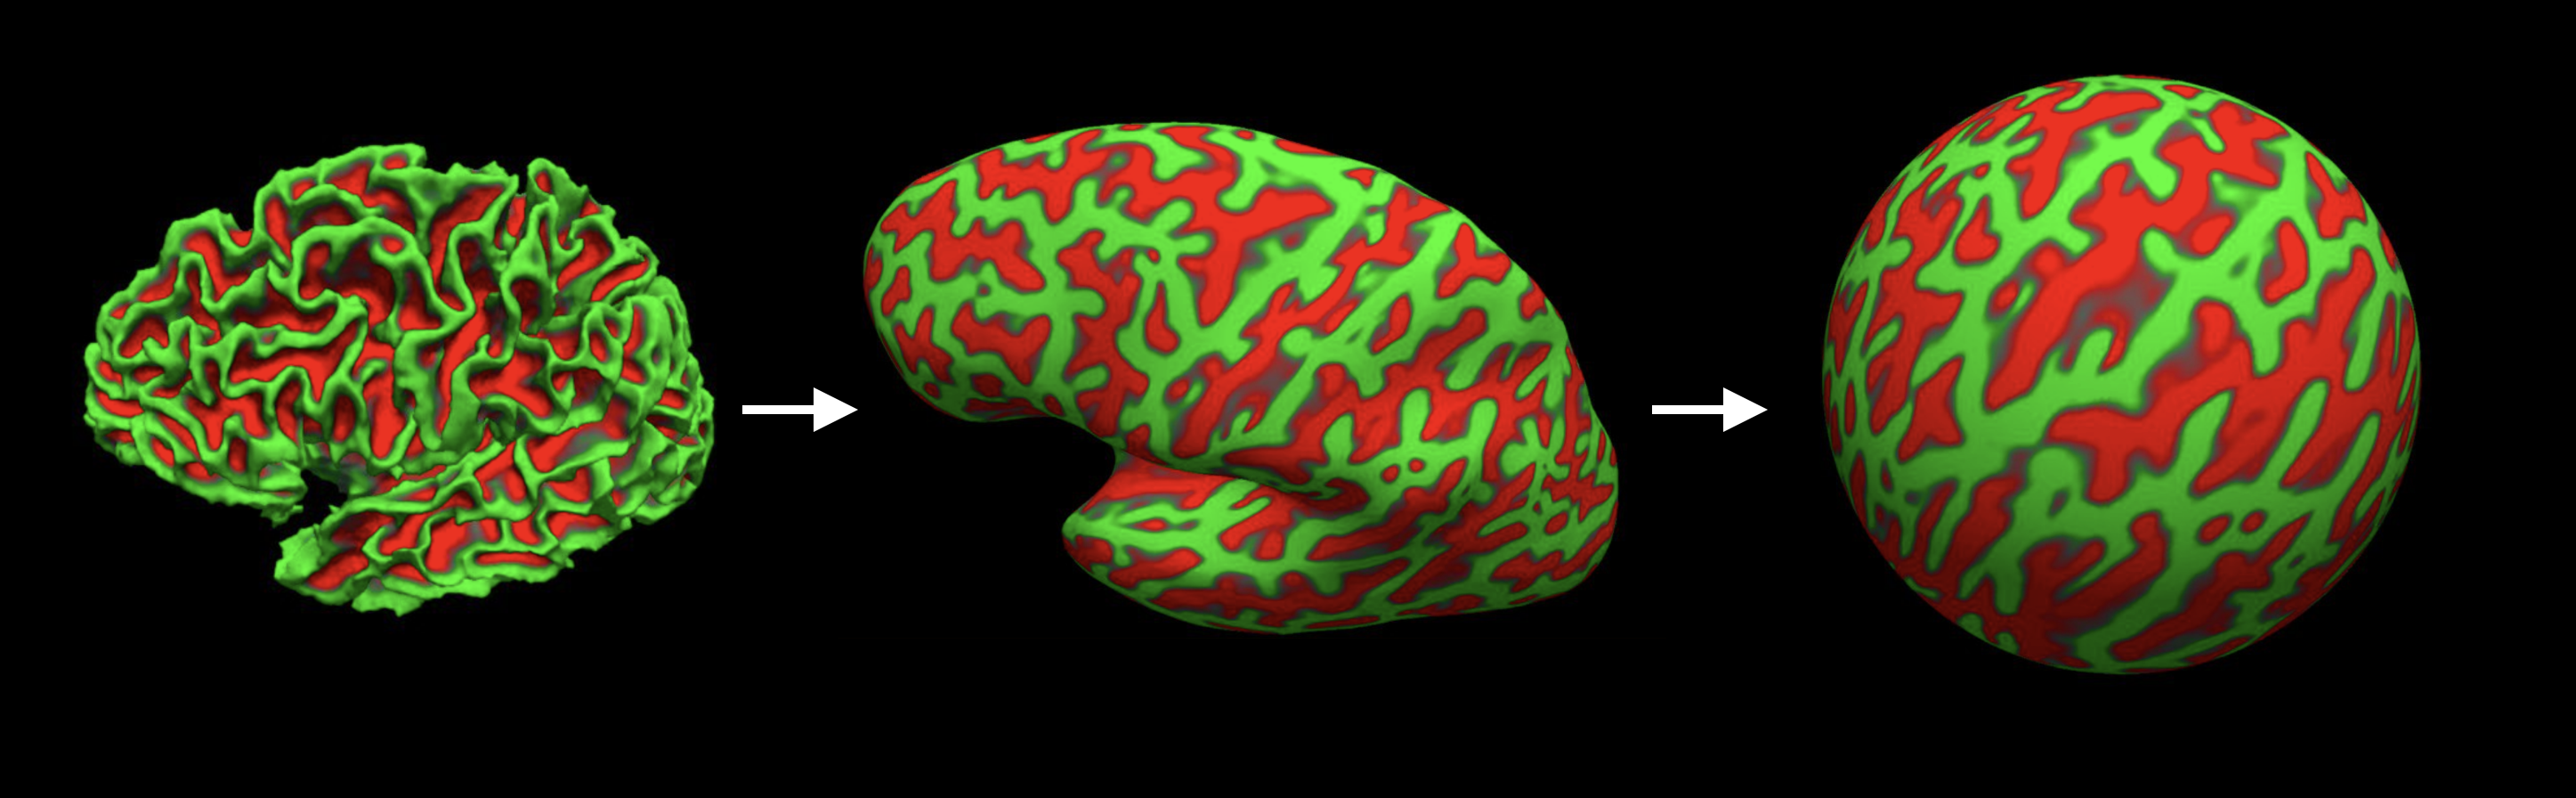
\includegraphics[width=0.8\textwidth]{image/pic2.png}
        \caption{
          The process of transforming brain geometry into a spherical representation using the inflation procedure.
        }
    \end{figure}

    The identified defects are then corrected using local algorithms that take into account the intensity profile of
    the original MRI image, allowing for the restoration of correct surface topology without the loss of meaningful
    cortical regions \cite{acosta_2012}.

    \item Once a topologically correct inner surface of the brain has been obtained, the outer (pial) surface —
    representing the external boundary of the gray matter — is reconstructed. This is achieved by progressively
    deforming the inner surface outward until it reaches the interface between gray matter and cerebrospinal fluid,
    again using the adaptive algorithms described above, which account for both signal intensity variations and
    cortical folding curvature. As a result of this stage, two mutually aligned surfaces (the gray–white matter
    boundary and the pial surface) are formed, enabling precise computation of cortical thickness at any point on the
    cortical surface \cite{fischl_2008, fischl_2004}.

    \item  The final stage of the SBM pipeline is the morphometric analysis. The reconstructed surfaces are registered
    and mapped into a standard anatomical space, allowing for statistical comparisons across different subjects and
    groups. At this stage, the following parameters are computed using numerical methods \cite{fischl_2000}:

    \begin{itemize}
      \item Cortical thickness is defined as the shortest distance between the white matter surface and the pial
      surface. For each point $p$ on the cortical surface, its local thickness is calculated as
      $T(p) = \text{dist}(S, S_{\text{pial}})$.
    
      \item Cortical volume is computed as the surface integral of cortical thickness over the pial surface:
      $V = \int T(p) \, dS$.
    
      \item Surface area is calculated as the surface integral over the pial surface: $A = \int dS$. \newline
    \end{itemize}
\end{enumerate}

\begin{figure}[H]
    \centering
    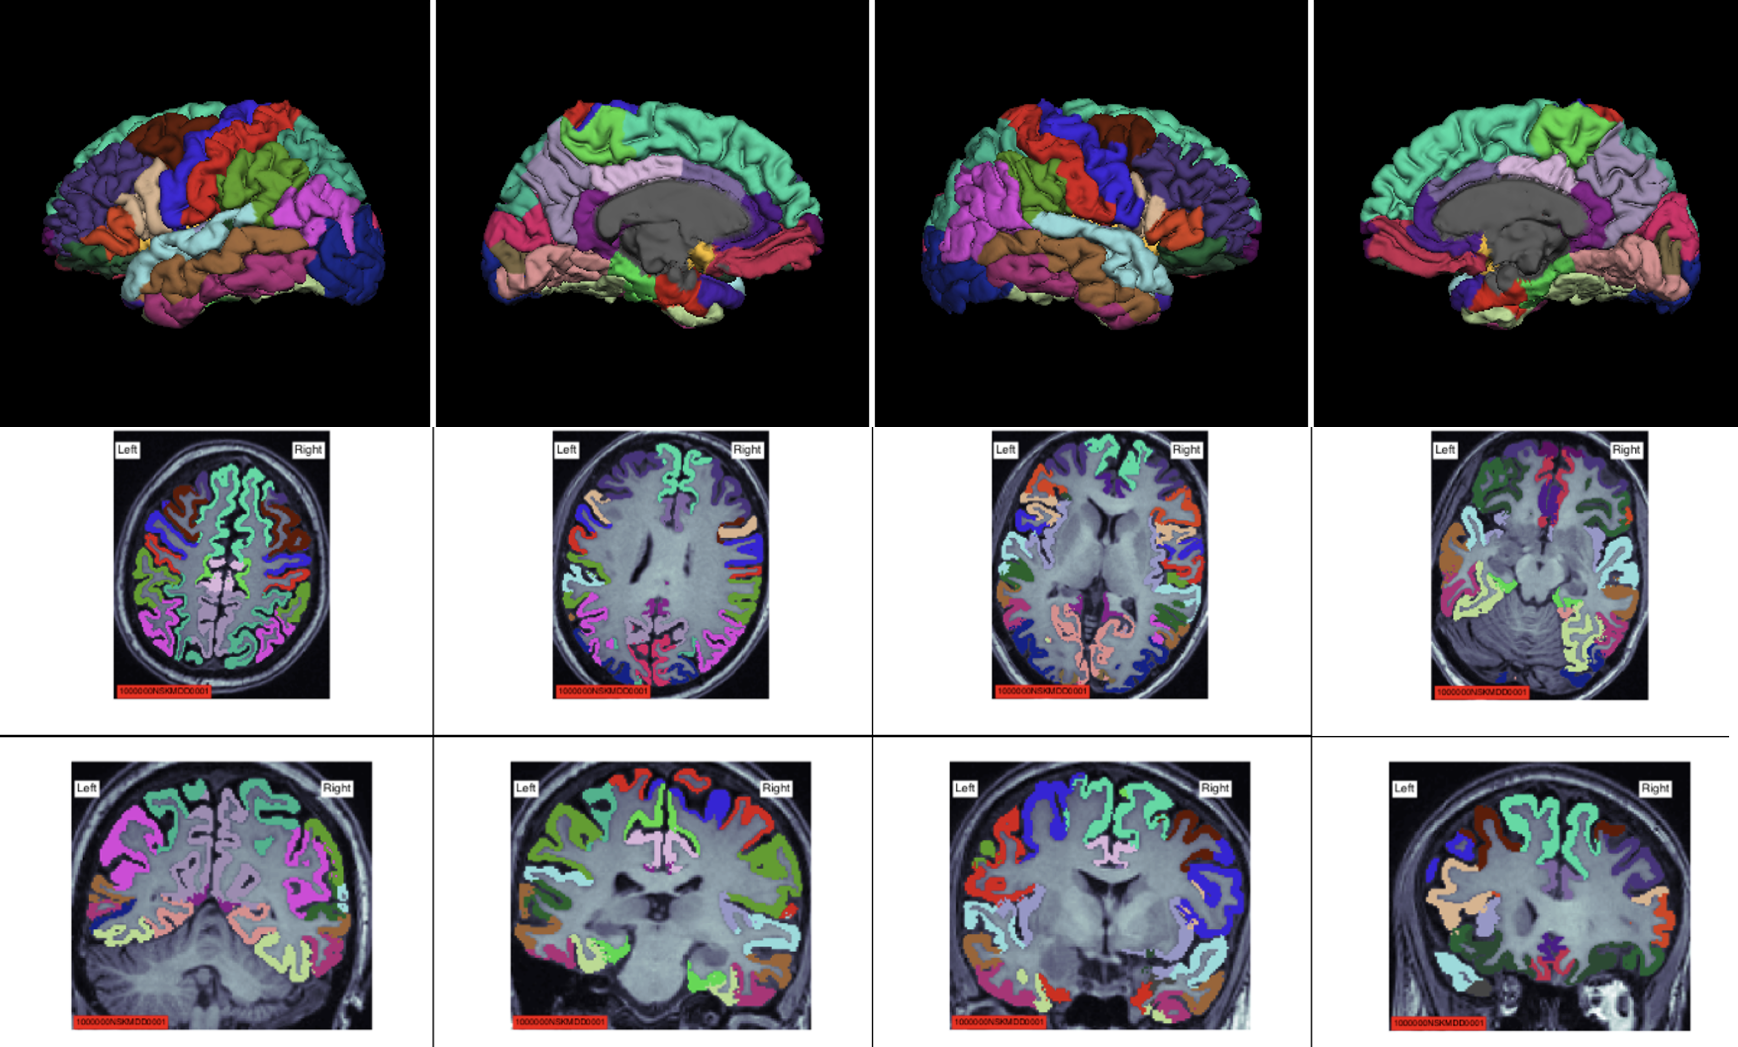
\includegraphics[width=0.8\textwidth]{image/pic3.png}
    \caption{
      Example of SBM application in the analysis of individual variability in cortical structures in patients
      with major depressive disorder: lateral and medial views (a); axial and coronal views (b).
    }
\end{figure}

The accuracy of this method reaches a level of less than a quarter of a millimeter, ensuring high reproducibility and
sensitivity to changes that may reflect age-related, pathological, or neuropsychological characteristics of the
cerebral cortex.

Below are the main parameters and metrics analyzed using SBM:\newline

\begin{itemize}
    \item Cortical thickness - the most commonly used SBM parameter, calculated as the distance between the gray–white
    and gray–CSF boundaries of the cortex \cite{evans_2015}. It is used, for example, to study age-related changes,
    neurodegenerative diseases (including Alzheimer’s disease), and neuroplasticity.
    
    \item Surface area - reflects both the developmental and individual characteristics of the brain structure.
    
    \item Gyrification index \cite{madeira_2020} — quantifies the degree of cortical folding and is calculated as the
    ratio of the total pial (folded) surface area to the area of its convex hull: $GI = \frac{A}{A_{\text{conv}}}$
    \cite{zilles_1988}. This index is particularly relevant in studies of brain development and psychiatric disorders
    \cite{goto_2022}.
    
    \item Curvature — describes the shape of the cortex, including convexity and concavity. In \cite{fischl_2000},
    curvature is derived directly from the second derivative of the surface, which can be obtained using numerical
    methods \cite{meyer_2003}.\newline
\end{itemize}

Several variants of SBM can be distinguished, differing in the operations performed during morphometric
analysis:\newline
\begin{itemize}
    \item Classical approach \cite{fischl_2012}. Utilizes segmentation of T1-weighted images to build individual
    surface models; suitable for evaluating cortical thickness, surface area, and curvature.

    \item Statistical SBM with nonparametric testing \cite{pantazis_2004}. Employs analysis of displacement vector
    fields along with permutation testing to assess the significance of observed changes.

    \item Multimodal SBM \cite{goto_2022}. Integrates data from functional MRI, diffusion MRI, or metabolic imaging to
    enable a more comprehensive understanding of structure–function relationships.

    \item Morphometry of subcortical surfaces \cite{devanand_2012}. Applied to structures such as the hippocampus and
    amygdala, using 3D surface modeling and mesh node correspondence.\newline
\end{itemize}

\begin{figure}[H]
    \centering
    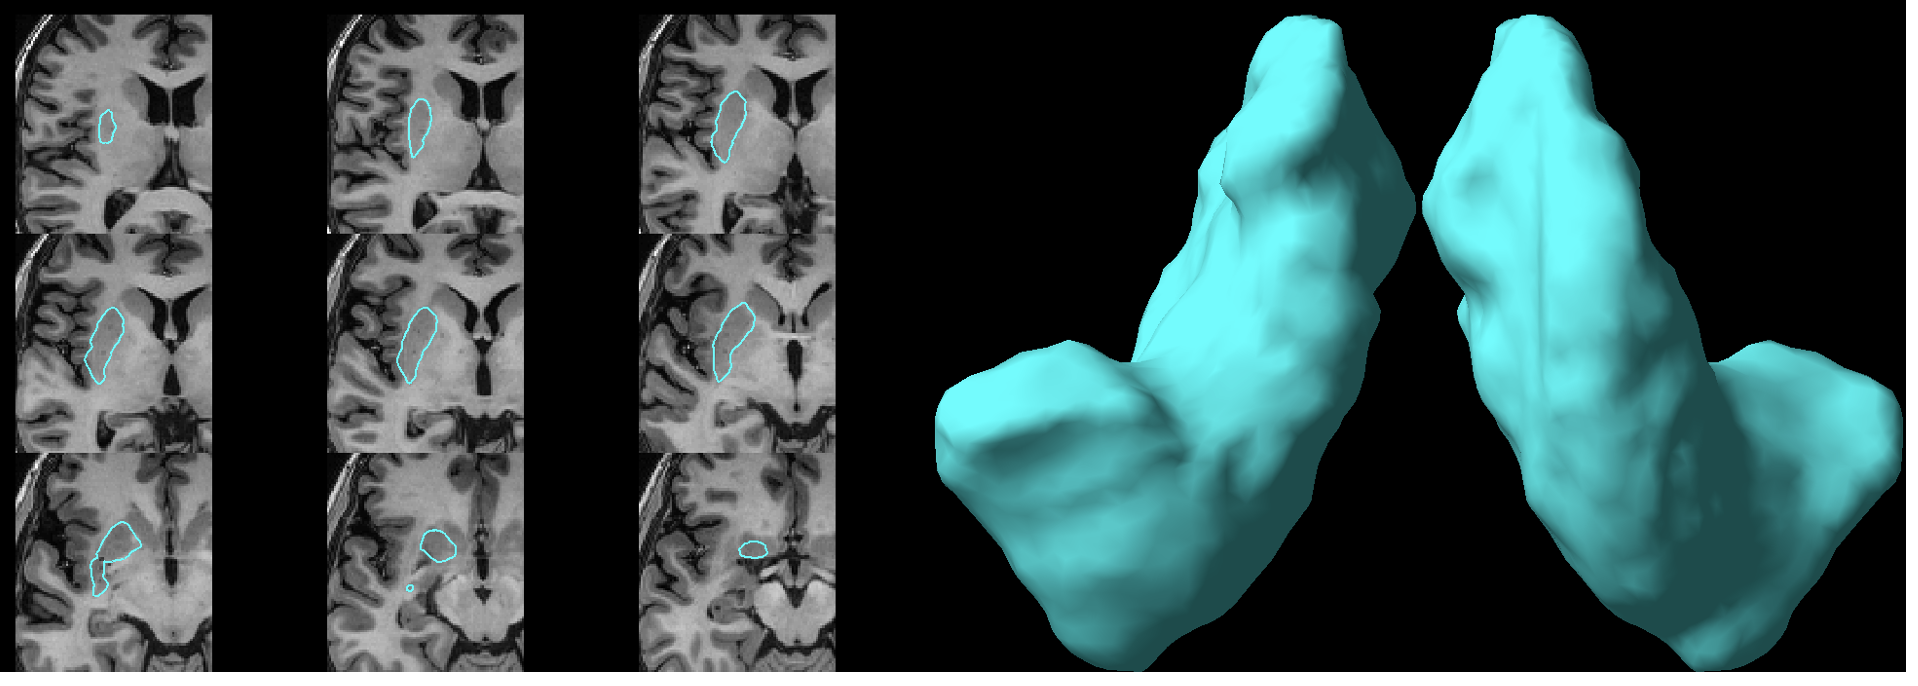
\includegraphics[width=0.8\textwidth]{image/pic1.png}
    \caption{
      Example of SBM application for analyzing individual variability in subcortical structures of the cerebral
      hemispheres in patients with major depressive disorder.
    }
\end{figure}

\subsection{Comparison of VBM and SBM}

The review article \cite{friston_2004} discusses the limitations of Voxel-Based Morphometry (VBM) in detecting
distributed brain changes due to its univariate analysis framework. The authors propose the use of multivariate models,
such as deformation-based morphometry, to better understand inter-regional dependencies within the brain.

The article also outlines the core characteristics of VBM, emphasizing its nature as a univariate approach that applies
statistical parametric mapping to spatially normalized brain images. VBM is designed to detect region-specific
structural differences in gray matter after spatial normalization, segmentation, and smoothing.

Importantly, the authors note that VBM is not intended for analyzing dependencies between different brain regions.
Rather, it identifies local differences in gray matter that are independent of changes in other areas. They also stress
that VBM does not replace shape analysis or provide detailed volumetric evaluation of well-defined anatomical
structures. In conclusion, the effectiveness of VBM in neuroanatomical research is acknowledged, but the authors argue
that analyzing complex spatial interactions requires multivariate approaches.

Surface-Based Morphometry (SBM), on the other hand, offers several substantial advantages over VBM, especially in the
context of cortical analysis \cite{evans_2015, friston_2004, voets_2008, lai_2020}:\newline

\begin{itemize}
    \item SBM accounts for the natural geometry and topology of the cortex, enabling more precise and biologically
    meaningful measurements of thickness, surface area, and curvature. In contrast, VBM operates in a volumetric space
    without respecting the specific characteristics of sulci and gyri, which reduces sensitivity to subtle local
    changes in cortical structure.
    
    \item SBM provides significantly better spatial registration of anatomical structures across subjects. This is
    achieved by projecting cortical surfaces onto a spherical model and precisely aligning folds and gyri, thereby
    minimizing inter-individual variability in cortical folding patterns. VBM, by contrast, relies on less sensitive
    normalization methods that are not well-suited for fine-scale cortical geometry, often resulting in suboptimal
    alignment between subjects.
    
    \item SBM exhibits higher sensitivity to small-scale changes in cortical thickness associated with both normal and
    pathological states. Since SBM enables direct measurement of cortical thickness as the distance between the pial
    surface and the gray-white boundary, it achieves submillimeter accuracy that VBM cannot provide.\newline
\end{itemize}

Thus, VBM does not utilize information about the specific shape of brain structures—only about their density and
volume. It may be susceptible to errors from inaccurate normalization or segmentation and relies on mass univariate
testing that ignores inter-regional dependencies \cite{ashburner_2000, mechelli_2005, callaert_2014}.

In contrast, SBM, due to its superior handling of cortical topology and geometry, more precise spatial registration,
and greater sensitivity to subtle morphometric changes, is considered the preferred method for detailed analysis of
cortical anatomy and is widely used in tools such as FreeSurfer \cite{fischl_2012}.

Additionally, in a study on traumatic brain injury, SBM demonstrated greater sensitivity than VBM in detecting
structural changes associated with neuropsychological test performance. This suggests that SBM may be a more accurate
approach for correlating brain anatomy with cognitive functions \cite{upadhyay_2014}.

\subsection{Accuracy of VBM and SBM Approaches}

Accuracy is a quantitative measure of how well a given approach can detect true morphometric differences between groups
or conditions (e.g., patients vs. healthy controls).
Several key metrics influence and define accuracy:\newline

\begin{itemize}
    \item Sensitivity – probability of a type I error (false positive)
    \item Specificity – probability of a type II error (false negative)
    \item Reproducibility – stability of results across repeated scans
    \item Spatial accuracy – how precisely the method localizes the effect\newline
\end{itemize}

The authors of study \cite{upadhyay_2014} claim that SBM has greater sensitivity to cortical changes. In a study
involving patients with traumatic brain injury, only SBM was able to detect significant correlations between cortical
thickness and cognitive test performance, while VBM did not. This indicates a higher sensitivity of SBM in cortical
structure analysis.

Furthermore, study \cite{friston_2004} demonstrated that the accuracy of VBM is highly dependent on the quality of
spatial normalization and smoothing \cite{han_2006}. Errors at these stages can blur local changes and reduce spatial
precision, which limits the reliability of VBM-based findings.

Lastly, the review study \cite{goto_2022} shows that SBM is more accurate in measuring cortical thickness and
gyrification, whereas VBM may be more effective for assessing subcortical and global volumetric changes. The authors
conclude that the best practice is to use both methods in combination for a comprehensive assessment.

A comparison table summarizing the analytic properties of the reviewed morphometric methods is presented below.

\begin{longtable}{|>{\bfseries}p{2.9cm}|p{4.5cm}|p{4.5cm}|}
\hline
Characteristic & \textbf{VBM} & \textbf{SBM} \\
\hline
\endfirsthead

\hline
\textbf{Characteristic} & \textbf{Voxel-Based Morphometry} & \textbf{Surface-Based Morphometry} \\
\hline
\endhead

\hline
\endfoot

\hline
\endlastfoot

Analysis space & Volume (3D voxels) & Surface (vertices, polygons) \\
\hline
Measured parameters & Density, gray matter volume & Thickness, area, curvature, gyrification \\
\hline
Accuracy & Lower for cortical analysis, sensitive to registration and input data & Higher for cortical analysis \\
\hline
Application & Assessment of overall volumetric changes & Detailed cortical analysis — thickness, curvature,
“gyrification” \\
\hline
Software tools & SPM, FSL & FreeSurfer, BrainVISA, CIVET \\
\hline
Robustness to geometry distortions & Lower, especially due to nonlinear normalization & Higher, as analysis is
performed on the native cortical geometry \\
\hline
Computational load & Lower & Higher; requires more time and resources due to complex surface reconstruction \\
\hline
Anatomical accuracy in cortical analysis & Limited (surface features not accounted for) & High, as analysis is
performed directly on the cortex \\
\hline
Sensitivity to local morphological changes & Lower, especially after smoothing & Higher, due to direct surface and
curvature-sensitive smoothing \\
\hline
Applicability in brain studies & Suitable for identifying global volumetric changes & Preferable for detecting subtle
structural changes in the cortex \\
\hline
\end{longtable}

\section{Multiscale Approach}

The study by \cite{cao_2023} introduces a method implementing tensor-based surface morphometry (TBSM), a modern
approach for analyzing structural changes in the cerebral cortex. TBSM is based on concepts from differential geometry
and tensor calculus, allowing for direct examination of geometric changes in the cortical surface while avoiding
distortions inherent in traditional methods that require surface flattening.

The TBSM processing pipeline begins with automatic segmentation of cortical surfaces from T1-weighted MRI scans, which
are pre-classified into gray matter, white matter, and cerebrospinal fluid. These surfaces are then modeled as
continuous triangular meshes, followed by a mathematical description of surface deformation over time. A key
innovation is the use of tensor geometry, which enables the computation of local changes in surface area, cortical
thickness, and curvature.

A core advantage of TBSM is its ability to measure local changes in morphometric parameters directly on cortical
surfaces with high sensitivity. The approach also incorporates diffusion-based smoothing on cortical surfaces, which
improves the signal-to-noise ratio and enhances the accuracy of statistical inference. As a result, TBSM enables
precise localization of areas with significant cortical thickness increases or decreases, as well as changes in
curvature and surface area — particularly relevant for studies of brain development and neurodegenerative diseases.

Tensor-based surface morphometry (TBSM) differs from traditional surface-based morphometry (SBM) in both its
mathematical framework and data analysis methods. While SBM uses classical geometry to reconstruct the cortical
surface and evaluate parameters such as thickness, area, and curvature, TBSM relies on more advanced differential
and tensor geometry. This allows deformations to be described using tensors, providing greater precision in
investigating both local and global changes in brain shape.

Moreover, TBSM avoids distortions typical of traditional methods: in SBM, complex cortical structures are often
projected onto simplified forms (e.g., a sphere), which can distort geometric properties \cite{chung_2002}. In
contrast, TBSM analyzes data directly on the original cortical surface, without simplification, reducing error and
enabling more accurate registration.

An additional advantage of TBSM is its heightened sensitivity to subtle morphometric changes. Thanks to diffusion-based
smoothing adapted to curved surfaces, this method allows for more precise localization and quantitative assessment of
even small changes in cortical shape and thickness — capabilities that are unattainable with standard smoothing in SBM.

Finally, the tensor-based framework of TBSM enables the integration of multiple morphometric characteristics — cortical
thickness, curvature, surface area, and volume — into a single analytical model. In traditional SBM, these parameters
are typically analyzed separately, which limits the comprehensiveness of the analysis.

Thus, TBSM represents a more advanced analytical method, providing more precise and reliable characterization of
structural changes in the cerebral cortex by employing a tensor-based approach and preserving the natural geometry
of cortical surfaces.

\section{Conclusion}

The main approaches to reconstructing the volumetric geometry of the cerebral cortex based on magnetic resonance
imaging have been reviewed. Particular attention was given to the comparative analysis of voxel-based morphometry
(VBM) and surface-based morphometry (SBM), their respective advantages and limitations, as well as to the prospects
of applying modern techniques such as tensor-based surface morphometry (TBSM).

It has been shown that SBM provides more accurate and anatomically meaningful results due to its consideration of
the natural topology and geometry of cortical structures. It also demonstrates increased sensitivity to subtle
morphometric changes. At the same time, the emerging TBSM approach offers advantages in mitigating geometric
distortions inherent in traditional methods and allows for the integration of various morphometric metrics into a
unified analytical process.

\section{Future Work}

In future stages of this research, an analysis of automated methods for reconstructing brain white matter tracts —
TRACULA, AFQ, and TractSeg — is planned, with particular attention to probabilistic tractography constrained by
anatomical priors. Simultaneously, the study will address preprocessing steps for diffusion-weighted imaging, including
motion artifact correction, eddy current compensation, and both affine and non-linear transformations. As a result,
quality criteria for input data will be formulated.

The experimental part will include the reconstruction of structural models across several datasets using the NextBrain
atlas, automatic validation, and comparative analysis of the tracts. This will make it possible to identify the most
accurate and reproducible solutions suitable for practical applications.


\section{Acknowledgments}
\begin{funding}
  The work was conducted within the framework of the program “Priority-2030”, of the Ministry of Science and Higher
  Education of the Russian Federation.
\end{funding}

\putbib[cite]

\makealttitle

\end{document}
